\documentclass[12pt]{extarticle}
\usepackage[utf8]{inputenc}
\usepackage{graphicx}
\usepackage{float}

% Disable indentation
\setlength{\parindent}{0pt}

\title{Lab 9: PKI HTTPS PROXY}
\author{Alexander Hoffmann \and Sofiane Rahli \and Yvan Compaore}
\date{\today}

\begin{document}

\maketitle

\section{Network configuration}
\textbf{1.} As we start the PC Router virtual machine, we need to modify the IP configuration. First, enable the interface connected to the internet. To show all the available interfaces, use:
\begin{verbatim}
ip link
\end{verbatim}
\begin{center}
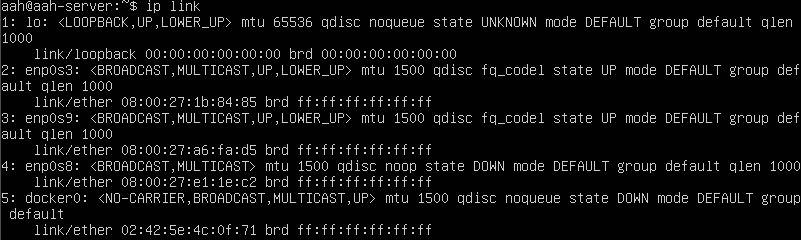
\includegraphics[scale=0.45]{resources/1-1-1.png}\\
\end{center}
There are 3 ip interfaces that interest us. \texttt{enp0s3} and \texttt{enp0s9} are host-only adapters. Observe that interface \texttt{enp0s8} is down. It corresponds to the NAT interface in the VirtualBox network configuration. We need to enable the interface and assign it an IP address using DHCP.
\begin{verbatim}
ifconfig enp0s8 up
\end{verbatim}
Now the interface is enabled but it does not have an IP address. To ask for a new DHCP lease, use:
\begin{verbatim}
dhclient enp0s8
\end{verbatim}
Now the DHCP sent a lease and the interface now has an IP address and an active internet connection.
\begin{center}
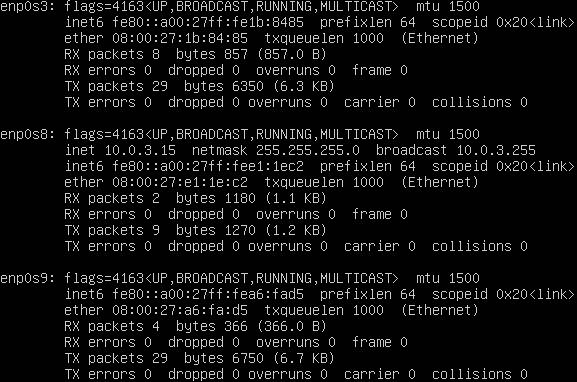
\includegraphics[scale=0.6]{resources/1-1-2.png}\\
\end{center}
To prove that the VM is connected to the internet, we ping the \texttt{google.com} server.
\begin{center}
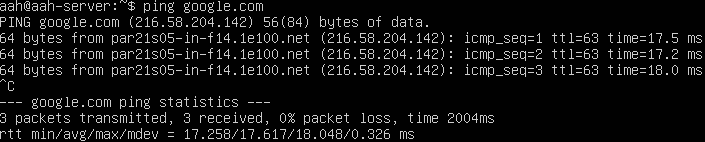
\includegraphics[scale=0.5]{resources/1-1-3.png}\\
\end{center}

\textbf{2.} 
Set the IP addresses of the other devices in the network using:
\begin{verbatim}
ifconfig <interface> <ip-address> netmask <netmask> up
\end{verbatim}
To add a default gateway to a network interface, use:
\begin{verbatim}
route add default gw <ip-address>
\end{verbatim}
\begin{table}[H]
\begin{tabular}{|l|l|}
\hline
\multicolumn{1}{|c|}{\textbf{VM}} & \multicolumn{1}{c|}{\textbf{IP Address}} \\ \hline
PC1                               & 192.168.11.2                             \\ \hline
PC2                               & 192.168.22.2                             \\ \hline
Server                            & 192.168.11.3                             \\ \hline
\end{tabular}
\end{table}

\section{CA ROOT}
\textbf{1.} Connect to PC2.\\

\textbf{2.} Here is a screenshot of the file structure.
\begin{center}
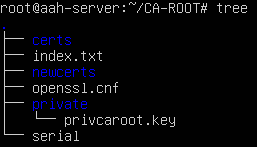
\includegraphics[scale=0.7]{resources/2-2-1.png}\\
\end{center}

\textbf{3.} To generate a private RSA key, use:
\begin{verbatim}
openssl genrsa -out privcaroot.key -des3 2048
\end{verbatim}

\textbf{4.} To create a self-signed certificate:
\begin{verbatim}
openssl req -new -x509 -days 365 -key private/privcaroot.key -out
certs/certcaroot.crt -config ./openssl.cnf -extensions CA_ROOT
\end{verbatim}
\begin{center}
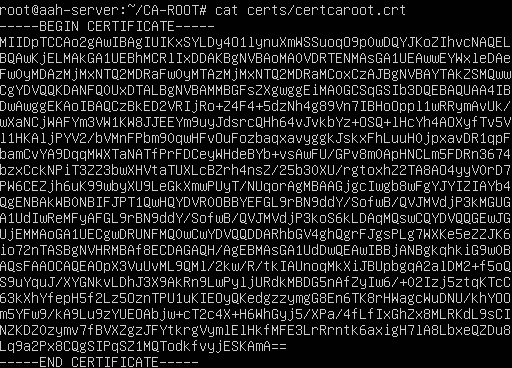
\includegraphics[scale=0.7]{resources/2-2-4.png}\\
\end{center}
\begin{center}
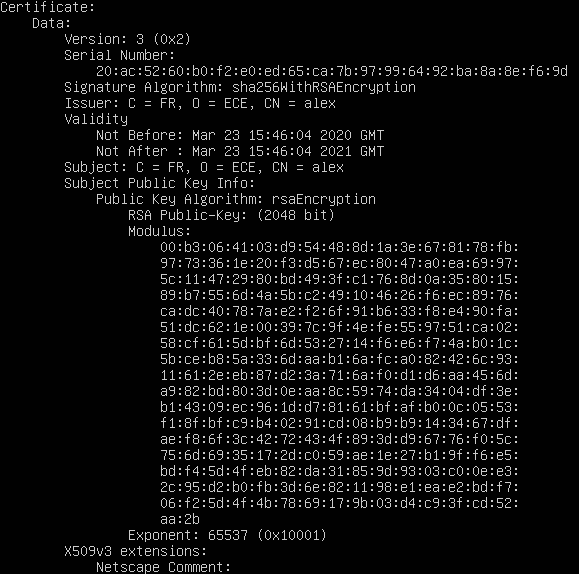
\includegraphics[scale=0.7]{resources/2-2-5.png}\\
\end{center}

\section{CA LAB}
\textbf{3.} Generate private RSA key.
\begin{verbatim}
openssl genrsa -des3 -out private/privcalab.key 2048
\end{verbatim}

\textbf{4.} Generate certificate.
\begin{verbatim}
openssl req -new -key private/privcalab.key -out certs/certcalab.csr
-config ./openssl.cnf
\end{verbatim}

\end{document}
